\documentclass[10pt]{beamer}

\usepackage[utf8]{inputenc}
\usepackage[swedish, english]{babel}
\usepackage{epstopdf}
\epstopdfsetup{update} % only regenerate pdf files when eps file is newer
\usepackage[squaren]{SIunits}

\usetheme[progressbar=frametitle]{metropolis}

\usepackage{booktabs}
\usepackage[scale=2]{ccicons}

\usepackage{pgfplots}
\usepgfplotslibrary{dateplot}

\usepackage{xspace}
\newcommand{\themename}{\textbf{\textsc{metropolis}}\xspace}

\usepackage{media9}

%\setbeamertemplate{frame footer}{Niklas Ericson - Linköping University}
\setbeamercolor{progress bar}{ fg = CERNBlue , bg = CERNBlue!30 }
\setbeamercolor{alerted text}{ fg = CERNBlue , bg = CERNBlue!30 }

\title{Presentation of Master's Thesis}
\subtitle{Investigation of Control Approaches for a High Precision, \\ Piezo-actuated Rotational Stage}
\date{\today}
\author{Niklas Ericson}
\institute{Linköping University | European Organization for Nuclear Research}
\titlegraphic{\hfill
\includegraphics[height=1cm, trim=0cm 0.65cm 0cm 0cm, clip=true]{../fig/LiU_primary_black}
              \hspace{0.2cm}
\includegraphics[height=1.2cm]{../fig/CERNLogoBadge}}

\begin{document}

\maketitle

\begin{frame}{Table of contents}
  \setbeamertemplate{section in toc}[sections numbered]
  \tableofcontents[hideallsubsections]
\end{frame}

\section{Introduction}

\begin{frame}[fragile]{CERN}
  The Large Hadron Collider (LHC) at CERN.
\center
\includemedia[
  width=0.8\linewidth,height=0.5\linewidth,
  activate=pageopen,
  flashvars={
    modestbranding=1 % no YT logo in control bar
   &autohide=1       % controlbar autohide
   &autoplay=1
   &cc_load_policy=1
   &showinfo=0       % no title and other info before start
   &start=27
   &end=55
  }
]{}{http://www.youtube.com/v/h2-ocLjUhTU?rel=0}   % Flash file
Source: \cite{youtube}.
\end{frame}

\begin{frame}[fragile]{Collimation}
  Collimation system used in the LHC.
\center
\includemedia[
  width=0.8\linewidth,height=0.5\linewidth,
  activate=pageopen,
  flashvars={
    modestbranding=1 % no YT logo in control bar
   &autohide=1       % controlbar autohide
   &autoplay=1
   &cc_load_policy=1
   &showinfo=0       % no title and other info before start
   &start=76
   &end=121
  }
]{}{http://www.youtube.com/v/h2-ocLjUhTU?rel=0}   % Flash file
Source: \cite{youtube}.
\end{frame}

\begin{frame}[fragile]{Crystal Collimation}
  The UA9 collaboration at CERN investigates how bent crystals can be used to extract halo particles.

  \begin{figure}[h!]
    \centering %crop: left bottom right top
    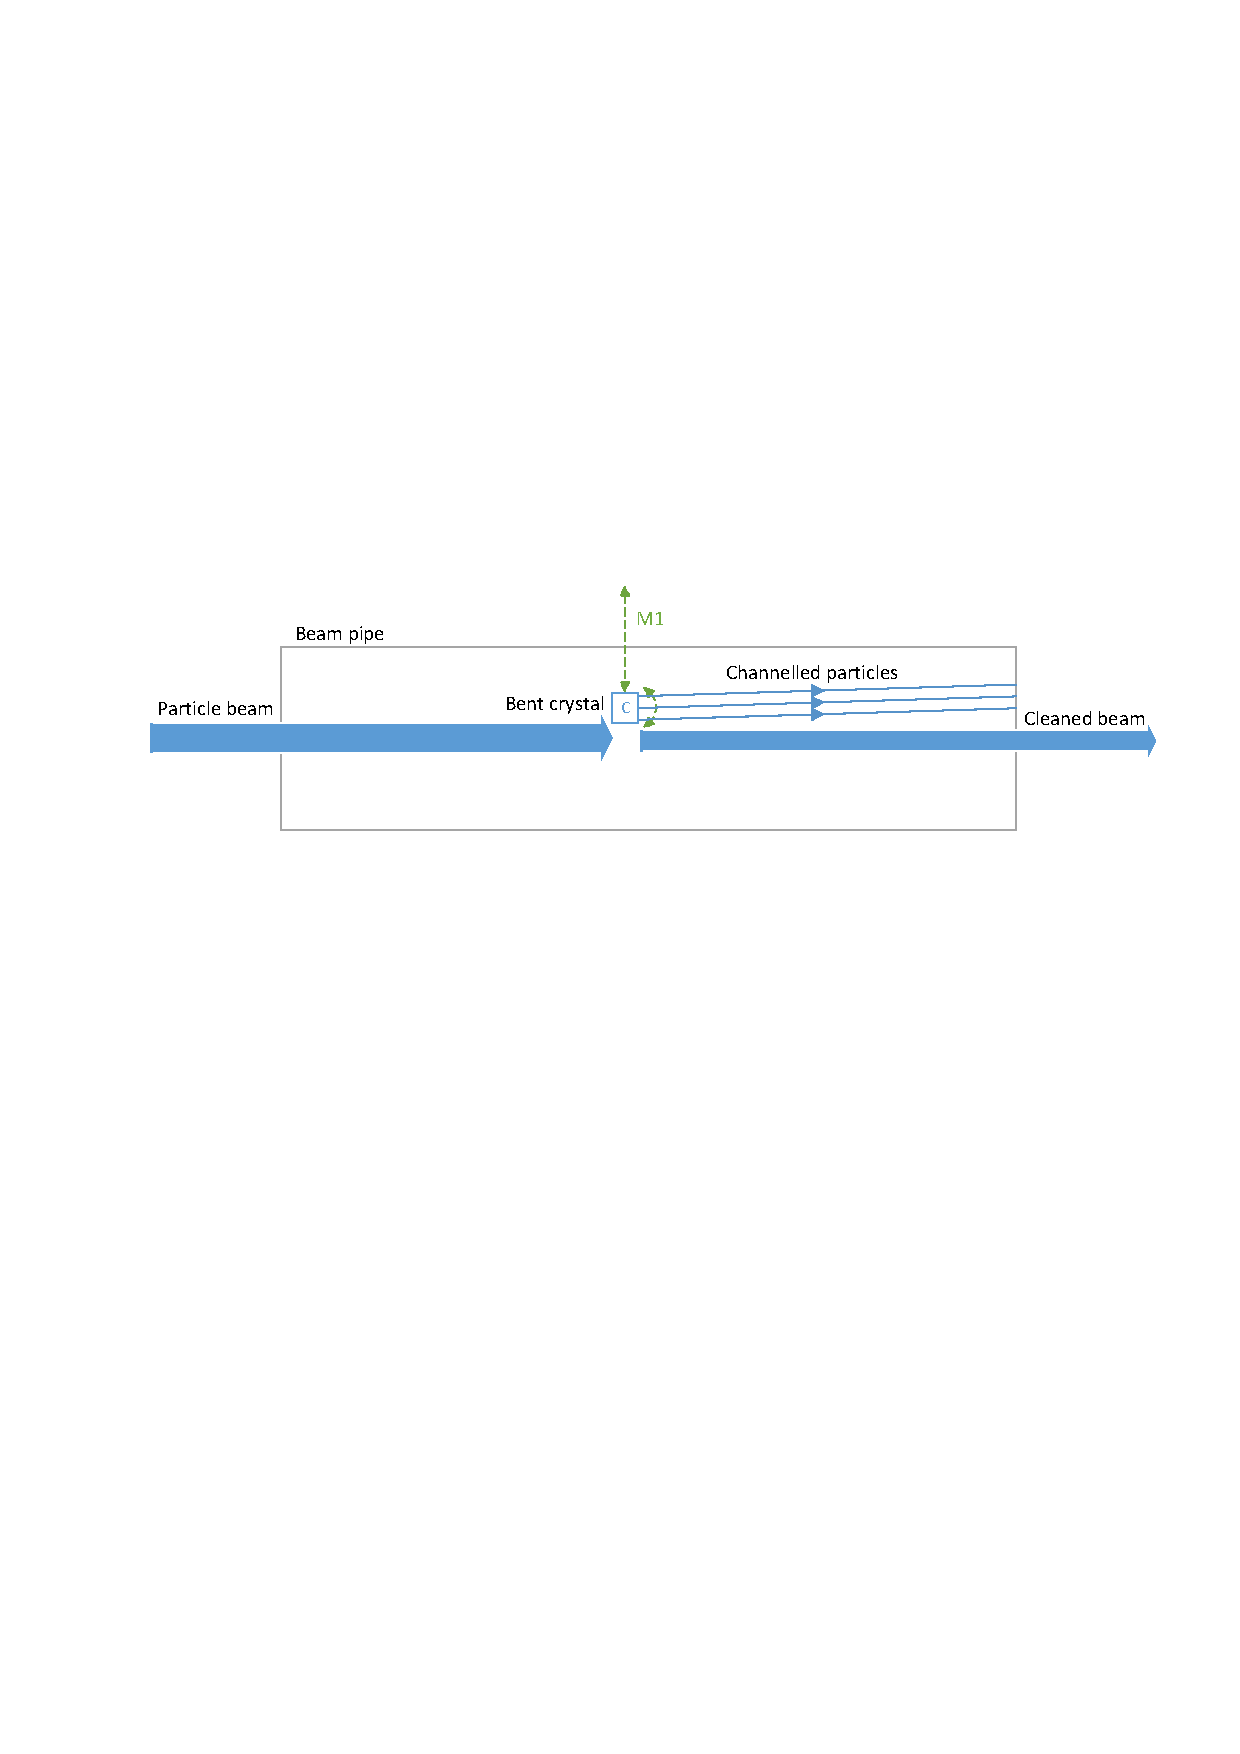
\includegraphics[width=1\textwidth, trim= 2cm 15.5cm 1cm 10cm, clip=true]{../fig/matlab/collimation}
    \caption{\label{fig:collimation}Illustration of the crystal collimation principle.}
  \end{figure}

  Implies in a more efficient cleaning, a less complex system and a reduction of the machine impedance.
\end{frame}


\begin{frame}[fragile]{Purpose and Goal}
  The \textbf{ higher the energy} of the particle the \textbf{lower the angular acceptance} for channeling.
  \begin{itemize}
    \item have a total range of \unit{20}{\milli\rad}
    \item be able to track reference trajectories at ramp rates of \unit{100}{\micro\radianpersecond}
    \item reject external disturbances to maintain a maximum tracking error of $\pm$\unit{1}{\micro\rad} even when the linear axis is moving
  \end{itemize}
\end{frame}

\begin{frame}[fragile]{Challenges}
  \begin{itemize}
    \item Nonlinear effect such as hysteresis and creep
    \item Highly resonant structure
    \item The linear movement adds additional perturbation
    \item System changes due to rotational and linear position, moving center of rotation.
  \end{itemize}
\end{frame}

\begin{frame}[fragile]{Method}
  Hello
\end{frame}

\section{System Overview}

\begin{frame}[fragile]{Crystal Collimators}
  The theme provides sensible defaults to \emph{emphasize} text,
  \alert{accent} parts or show \textbf{bold} results.
\end{frame}

\begin{frame}{Rotational stage}
  \begin{itemize}
    \item Regular
    \item \textit{Italic}
    \item \textsc{SmallCaps}
    \item \textbf{Bold}
    \item \textbf{\textit{Bold Italic}}
    \item \textbf{\textsc{Bold SmallCaps}}
    \item \texttt{Monospace}
    \item \texttt{\textit{Monospace Italic}}
    \item \texttt{\textbf{Monospace Bold}}
    \item \texttt{\textbf{\textit{Monospace Bold Italic}}}
  \end{itemize}
\end{frame}

\begin{frame}{Modeling}
\end{frame}

\begin{frame}{Present Control Approach}
  \begin{equation*}
    e = \lim_{n\to \infty} \left(1 + \frac{1}{n}\right)^n
  \end{equation*}
\end{frame}

\section{Approaches and Simulation Results}

\begin{frame}{Integral Resonance Control}
\end{frame}

\begin{frame}{Model Reference Adaptive Controller}
\end{frame}

\begin{frame}{Harmonic Cancellation}
\end{frame}

\begin{frame}{Comparison}
\end{frame}

\section{Implementation}

\begin{frame}{Setup}
\end{frame}

\begin{frame}{Experimental Results}
\end{frame}


\section{Conclusion}

\begin{frame}{Simulation Results}
\end{frame}

\begin{frame}{Experimental Results}
\end{frame}

\begin{frame}{Summary}
\end{frame}

\begin{frame}[standout]
  Questions?
\end{frame}

\appendix

\begin{frame}[allowframebreaks]{References}

  \bibliography{pres}
  \bibliographystyle{abbrv}

\end{frame}

\end{document}
